%!TEX root = ../../main.tex
\section{Administration Tools}\label{sec:designAdminTools}
In order for the administrator of the bicycle system to make reasonable decision about future actions/improvements towards the bicycle system, statistical data has to be collected and shown to the administrator. This will give him an overview of the usage of the bicycles and prepare him to possibly make a better decision or just provide him with a knowledge of how the system is used.
A list of questions should be able to be answered or hinted by the system, however, the implemented features in the final system will likely be limited by available time:

\begin{description}[style=nextline]
\item[Which routes are used?] If routes could be determined, patterns could possibly be seen, e.g. if there is a particular route that is very popular.\fxwarning{Patterns? Most popular?}
\item[Where is the most traffic of bicycles during some period?] An administrator would be able to see how many bicycles leaves and arrives at each station and thereby get an overview of where the traffic is high and low, providing an indication of where to put focus for relocation of bicycles and expansion of stations.
\item[What is the current amount of bicycles at a given station?] This gives the administrator an idea of when bicycles leave each station.
\item[How does the amount of bicycles at a given station change over time?] The administrator can choose a long time interval, providing a more general overview of when the activity at each station is high or low, also providing him with an overview of usage at each station.
\item[Are there hotspots for bicycles?] If positions of bicycles could be determined, it would mean that different kind of patterns could be detected, for example detecting stagnant bicycle hotspots could provide valuable knowledge about where to add new stations.
\end{description}

Keeping a log of information about the usage as described above, requires additional database tables having timestamps as an important factor since the usage of bicycles is tied to some real life events that needs to be logged. 
In order to log the routes for a bicycle, a new relation is added to the database schema storing information about longitude and latitude and of course which bicycle it is for and when it was logged.
In order to log traffic of bicycles between stations another relation is added to the schema having information about a start station and an end station for a trip along with times for each of the events (start of trip and end of trip).
Last, a relation to store the count of bicycles at each station along with a timestamp, is added to the schema.

Putting all this together, also illustrating foreign key references, can be seen in \figref{fig:er-dia-log}.

\begin{figure}
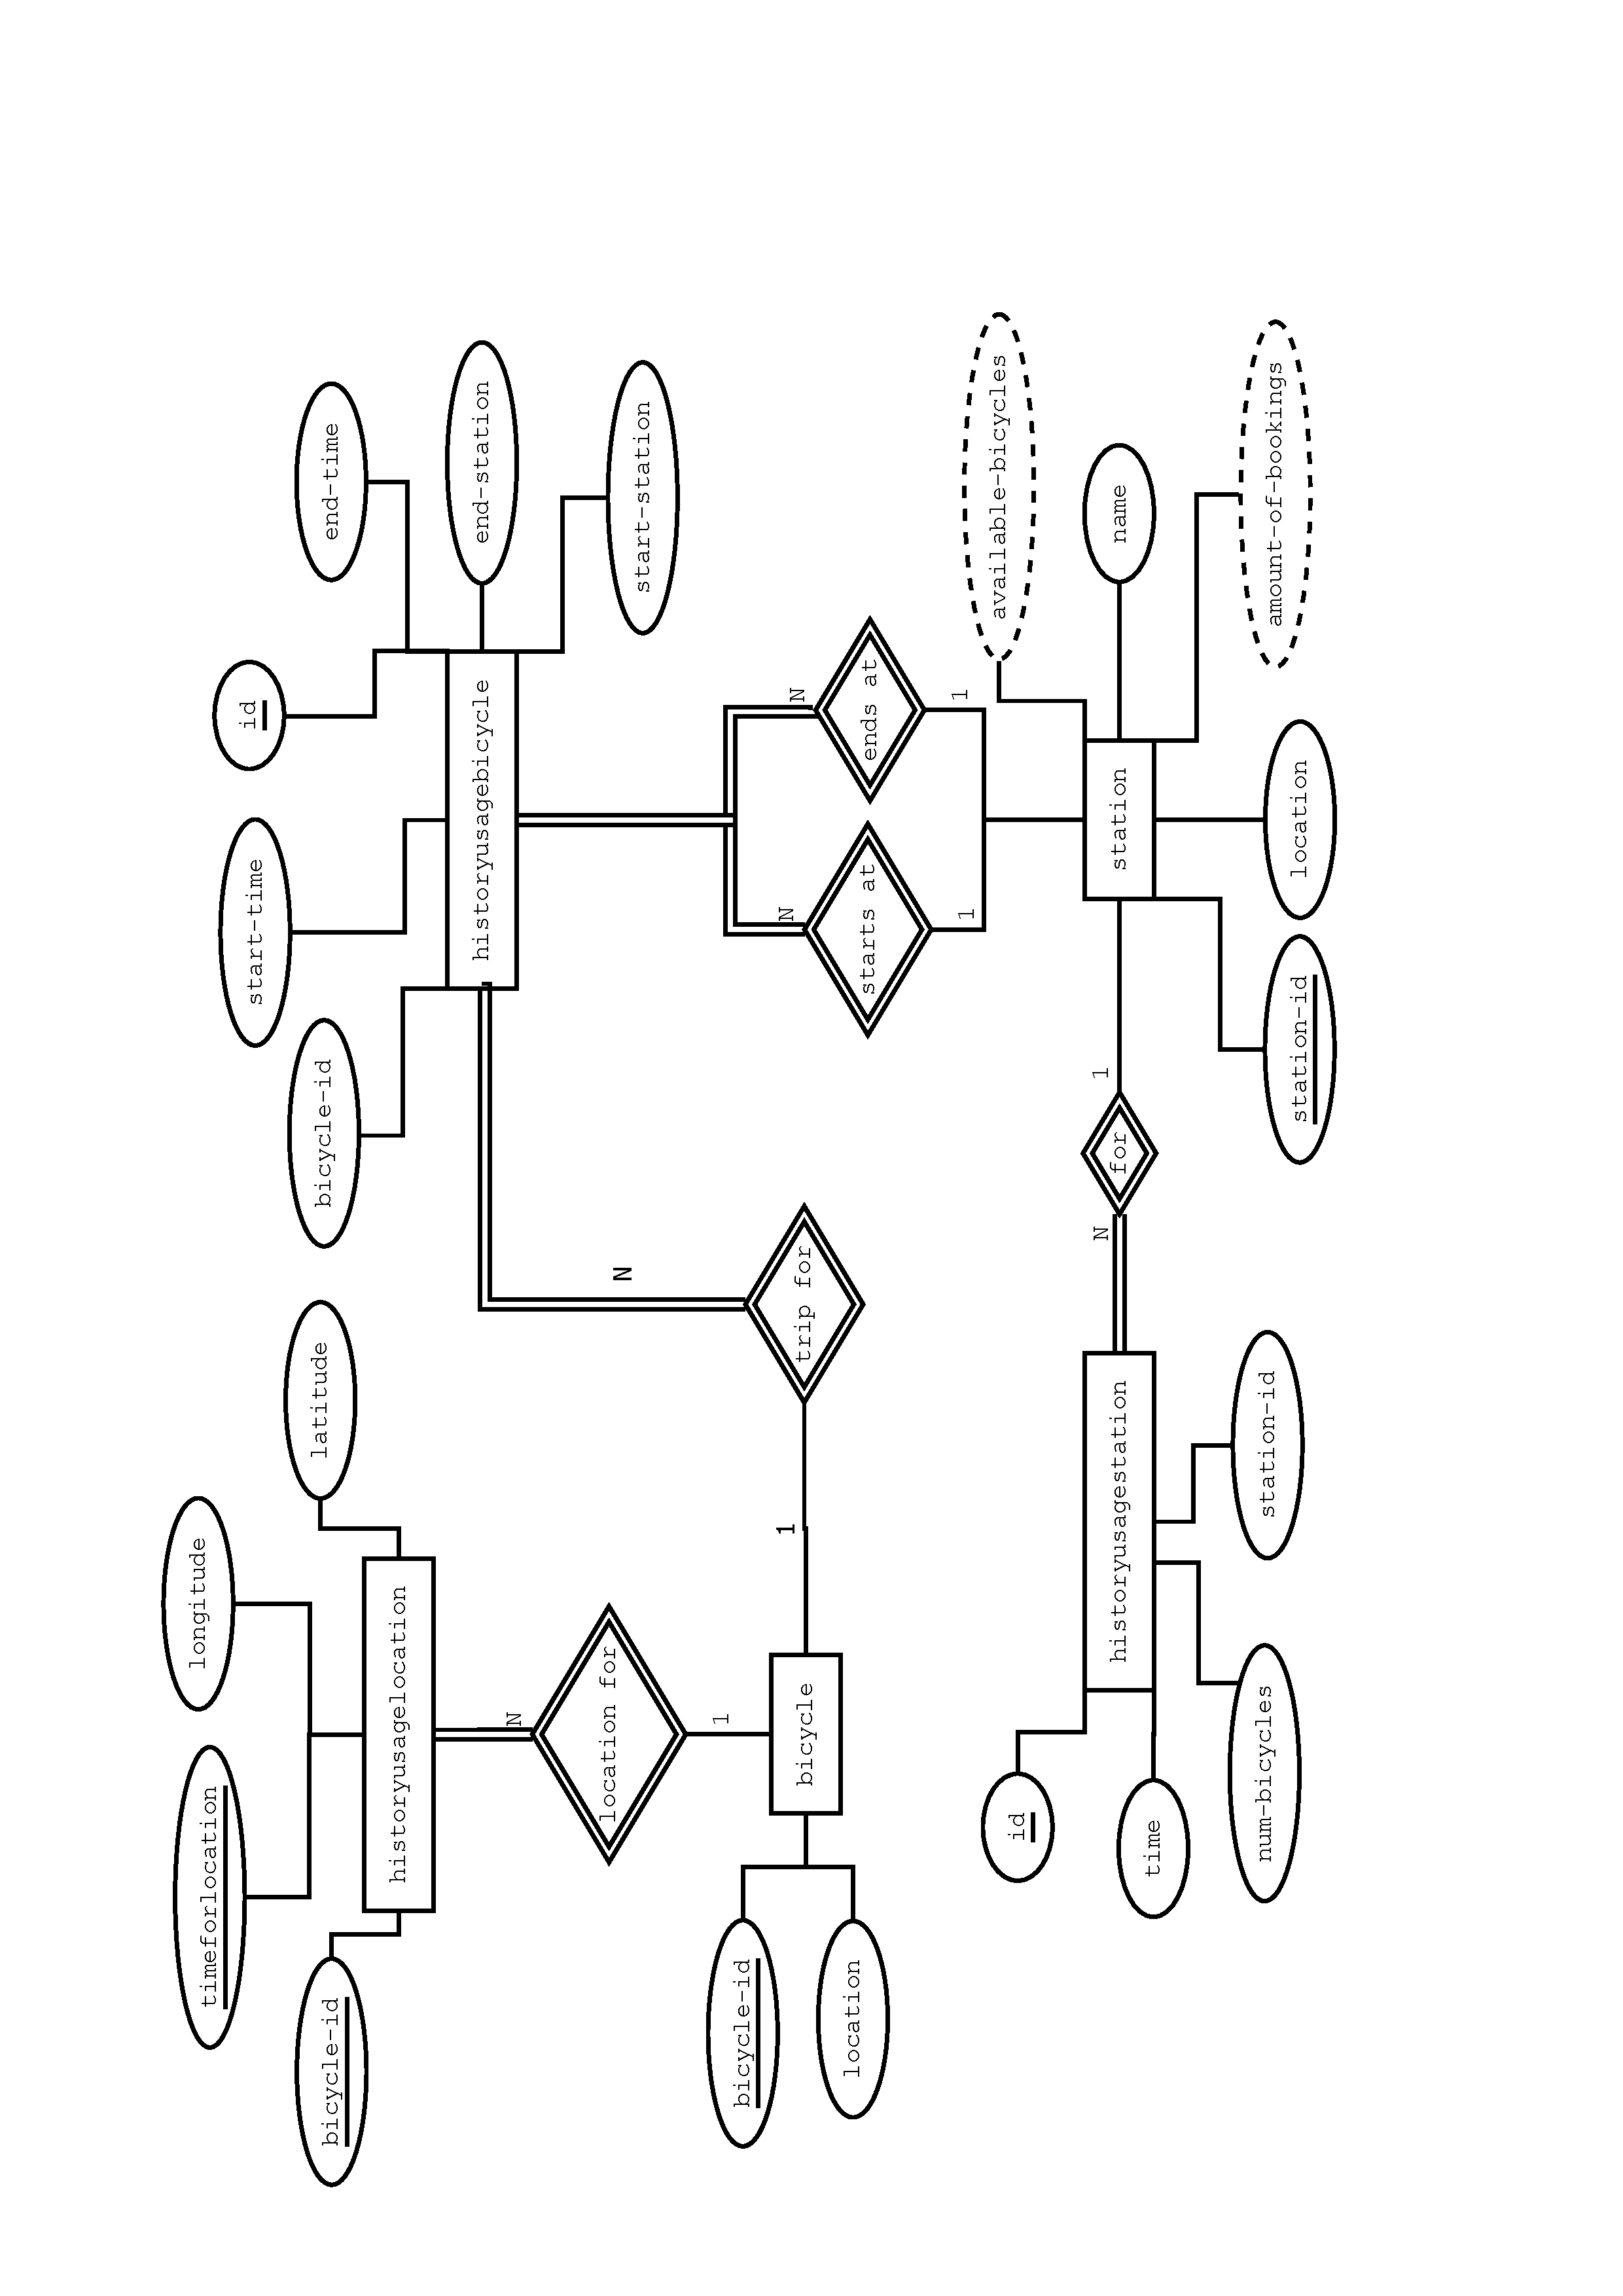
\includegraphics[scale=0.3, angle=-90]{design/ER-diagram-logging.pdf}
\vspace*{-2cm}
\caption{ER-diagram showing relations covering data logging.}\label{fig:er-dia-log}
\end{figure}

Addition and removal of bicycles, users, and stations is also part of the responsibility of the administration tools. 
For bicycles, they should be added to the system loosely and not directly to a station.
We intend to do it like this because when the administrator adds a new bicycle, they receive an id and the idea is that they use this id to program the bicycle such that it can be recognized by the system.
For users and stations, addition does not have any such considerations to make. 
The dock is not part of the administration tools, since it is handled station side.
For removal of stations, it is important that all bicycles at that station are released and that docks are deleted along with the station.

Since the logging tables use the other tables like the station and bicycle tables it is important to handle deletion of stations and bicycles. 
If deletion is not handled properly the logged data could end up being inconsistent. 
In our case we handle deletion by adding a column to the affected tables indicating if the row is deleted or not. 
When using the station and bicycles table on the website we make sure to only use the rows that is not deleted, while for the history data we use all rows.

An overview page of the stations should also be implemented, providing information about stations such as if they are online or not, where they are and what their status is with regards to usage.
